\tikzset{%
  every neuron/.style={
    circle,
    draw,
    minimum size=0.5cm
  },
  neuron missing/.style={
    draw=none, 
    scale=2,
    text height=0.333cm,
    execute at begin node=\color{black}$\vdots$
  },
}

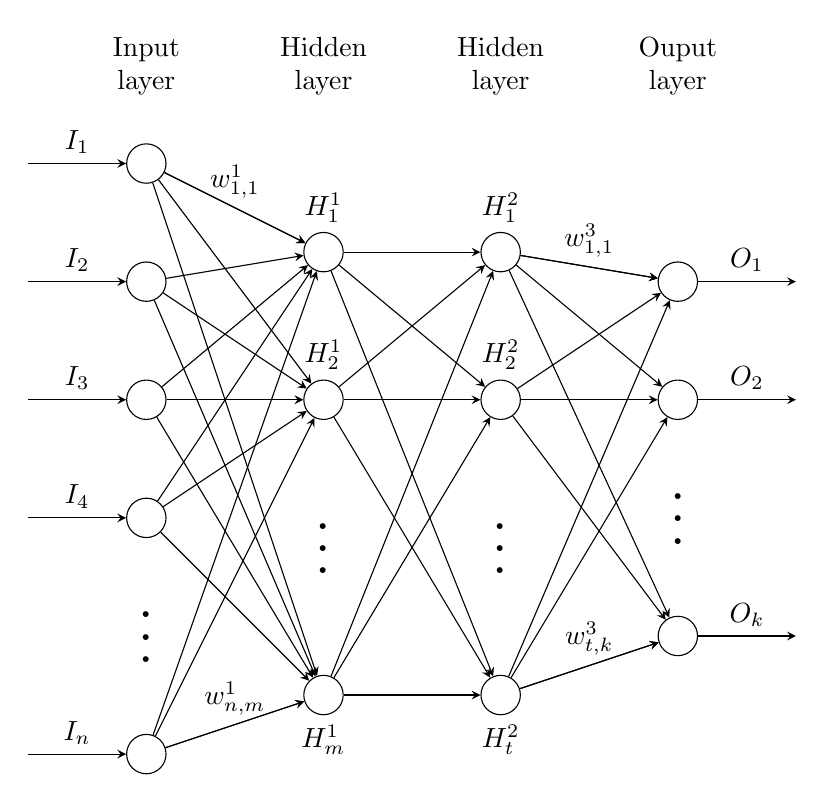
\begin{tikzpicture}[x=1.5cm, y=1.5cm, >=stealth]

    \foreach \m/\l [count=\y] in {1,2,3,4,missing,5}
      \node [every neuron/.try, neuron \m/.try] (input-\m) at (0,2.5-\y) {};
    
    \foreach \m [count=\y] in {1,2,missing,3}
      \node [every neuron/.try, neuron \m/.try ] (hidden1-\m) at (1.5,2-\y*1.25) {};
    
    \foreach \m [count=\y] in {1,2,missing,3}
      \node [every neuron/.try, neuron \m/.try ] (hidden2-\m) at (3,2-\y*1.25) {};
    
    \foreach \m [count=\y] in {1,2,missing,3}
      \node [every neuron/.try, neuron \m/.try ] (output-\m) at (4.5,1.5-\y) {};
    
    \foreach \l [count=\i] in {1,2,3,4,n}
      \draw [<-] (input-\i) -- ++(-1,0)
        node [above, midway] {$I_\l$};
    
    \foreach \l [count=\i] in {1,2}
      \node [above] at (hidden1-\i.north) {$H_\l^1$};
    
    \node [below] at (hidden1-3.south) {$H_m^1$};

    \foreach \l [count=\i] in {1,2}
      \node [above] at (hidden2-\i.north) {$H_\l^2$};
    
    \node [below] at (hidden2-3.south) {$H_t^2$};
    
    \foreach \l [count=\i] in {1,2,k}
      \draw [->] (output-\i) -- ++(1,0)
        node [above, midway] {$O_\l$};
    
    \draw [->] (input-1) -- (hidden1-1)
        node [above, midway] {$w_{1, 1}^1$};

    \draw [->] (input-5) -- (hidden1-3)
        node [above, midway] {$w_{n, m}^1$};

    \foreach \i in {1,...,5}
      \foreach \j in {1,...,3}
        \draw [->] (input-\i) -- (hidden1-\j);

    \draw [->] (hidden2-1) -- (output-1)
        node [above, midway] {$w_{1, 1}^3$};

    \draw [->] (hidden2-3) -- (output-3)
        node [above, midway] {$w_{t, k}^3$};

    \foreach \i in {1,...,3}
        \foreach \j in {1,...,3}
          \draw [->] (hidden1-\i) -- (hidden2-\j);
    
    \foreach \i in {1,...,3}
      \foreach \j in {1,...,3}
        \draw [->] (hidden2-\i) -- (output-\j);
    
    \foreach \l [count=\x from 0] in {Input, Hidden, Hidden, Ouput}
      \node [align=center, above] at (\x*1.5,2) {\l \\ layer};
    
    \end{tikzpicture}